% *******************************************************************************
% * Copyright (c) 2007 by Elexis
% * All rights reserved. This document and the accompanying materials
% * are made available under the terms of the Eclipse Public License v1.0
% * which accompanies this distribution, and is available at
% * http://www.eclipse.org/legal/epl-v10.html
% *
% * Contributors:
% *    G. Weirich
% *
% *  $Id: elexis-notes.tex 4855 2008-12-25 18:17:18Z rgw_ch $
% *******************************************************************************

\documentclass[a4paper]{scrartcl}
\usepackage{german}
\usepackage[utf8]{inputenc}
\usepackage{makeidx}
\makeindex

\usepackage[pdftex]{graphicx}
\DeclareGraphicsExtensions{.pdf,.jpg,.png}

\usepackage{floatflt}
\usepackage{wrapfig}
\usepackage[]{hyperref}
\usepackage{color}
\begin{document}
\title{Elexis-Notes}
\author{Gerry Weirich}
\maketitle

\section{Einführung}
Dieses Plugin dient dazu, beliebige nicht-patientenbezogene Informationen und Dokumente abzulegen. Diese können nach beliebigen Kriterien strukturiert und mit Stichwörtern versehen werden.

Ausserdem können, falls in Elexis ein Scanservice\footnote{Ein Scanservice liefert die Fähigkeit, Scanner anzusteuern und kann von einem anderen, separat zu besorgenden Plugin beigesteuert werden, z.b. Omnivore-direct ist ein solcher Service-Provider} vorhanden ist, Dokumente direkt eingescannt werden.

\medskip

elexis-notes benötigt Elexis ab Version 1.4

\section{Installation, Deinstallation, Konfiguration}
Wie üblich wird das Plugin durch einfaches Kopieren ins Plugins-Verzeichnis installiert und durch Löschen aus diesem Verzeichnis wieder deinstalliert.

\begin{figure}
  % Requires \usepackage{graphicx}
  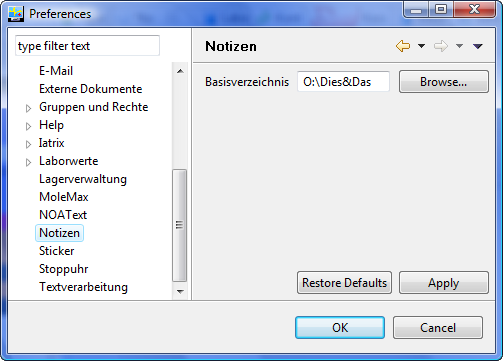
\includegraphics{config}\\
  \caption{Konfiguration}\label{fig:notes1}
\end{figure}

Die Konfiguration (Vgl. Abb. \ref{fig:notes1}) beschränkt sich darauf, ein Basisverzeichnis anzugeben, unterhalb dem  \textit{Elexis-Notes} externe Dokumente ablegen soll.

\section {Verwendung}
Wenn das Plugin korrekt installiert ist, finden Sie unter \textsc{Fenster-Views-Andere} eine View Namens 'Notizen' \ref{fig:notes}. Es sollte sich dann ein Fenster wie in Abb. \ref{fig:notes2} öffnen (natürlich zunächst ohne Inhalt).

\begin{figure}[htbp]
     \begin{minipage}{0.4\textwidth}
      \centering
       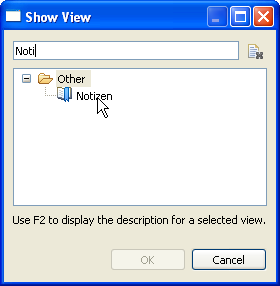
\includegraphics[width=0.8\textwidth]{notesview}
  \caption{View öffnen}\label{fig:notes}
     \end{minipage}\hfill
     \begin{minipage}{0.5\textwidth}
      \centering
       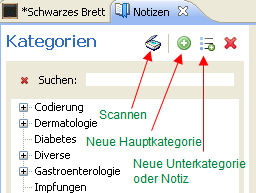
\includegraphics[width=0.8\textwidth]{notestools}
       \caption{Funktionen}
       \label{fig:tools}
     \end{minipage}
   \end{figure}



\begin{figure}
  % Requires \usepackage{graphicx}
  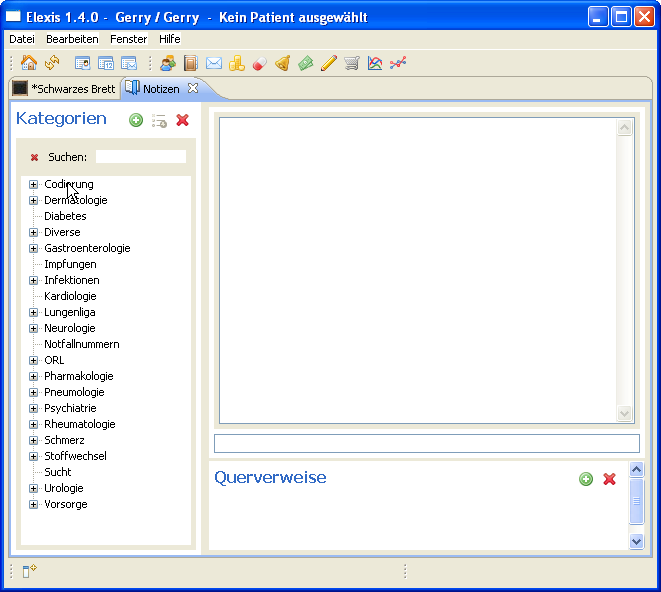
\includegraphics[width=0.9\textwidth]{notesview2}\\
  \caption{Notizen-View}\label{fig:notes2}
\end{figure}

\textit{Elexis-Notes} Ordnet Notizen und Dokumente beliebig hierarchisch. Sie können Hauptkategorien (die oberste Ebene) vorgeben und darunter beliebig viele Unterkategorieren in beliebig tiefer Schachtelung erstellen. Jede Unterkategorie kann gleichzeitig auch eine Notiz sein, resp. jede Notiz kann Unterkategorien enthalten.

\subsection{Neue Hauptkategorie erstellen}
Klick auf diesen Knopf öffnet ein Fenster um einen Namen einzugeben. Eine Hauptkategorie dieses Namens wird in der obersten Ebene er Liste erstellt.

\subsection{Neue Unterkategorie oder Notiz erstellen}
Klicken Sie auf die gewünschte Kategorie oder Notiz und klicken Sie auf diesen Button. Sie können dann wieder einen Namen eingeben, und der neue Eintrag wird unterhalb des vorher markierten Eintrags erstellt.

\subsection{Scannen}
Diese Funktion steht nur zur Verfügung, wenn Sie ein Plugin installiert haben, welches einen Scannerdienst anbietet (z.B. Omnivore direct). Markieren Sie eine gewünschte Kategorie oder Notiz und klicken Sie  auf den Scan-Button. Dies öffnet das Scanprogramm Ihres Scanners. Nach Einscannen des Dokuments können Sie einen Namen für das Dokument vergeben. Das Dokument wird dort abgespeichert, wo Sie in der Konfiguration das Basisverzeichnis angegeben hatten, und ein Verweis auf das Dokument wird unter dem markierten Eintrag angelegt.

\subsection{Notizen schreiben}
Im rechten Feld können Sie beliebig Text eingeben, der dem links markierten Element (Kategorie, Unterkategorie oder Notiz) zugeordnet wird. Bei Verlassen des Feldes wird der Text automatisch gespeichert.

\subsection{Externe Dokumente oder Websites verlinken}
Im unteren Feld können Sie mit Klick auf den + Button Links erstellen. Ein Link kann entweder eine beliebige Datei oder ein Internet-Link sein (Komplett mit http:// einzugeben). Vgl Abb. \ref{fig:notes3}.

\begin{figure}
  % Requires \usepackage{graphicx}
  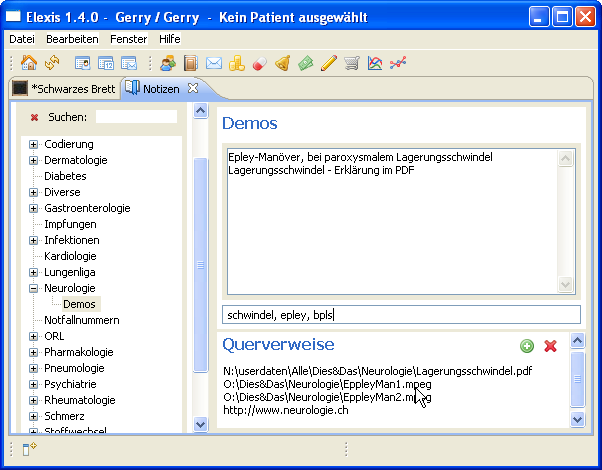
\includegraphics[width=0.8\textwidth]{notesview3}\\
  \caption{Beispiel für einen Eintrag}\label{fig:notes3}
\end{figure}

\subsection{Stichwörter zuordnen}
Im mittleren Feld zwischen Titel und Querverweisen können Sie beliebige, durch Komma getrennte Stichwörter zur aktuellen Notiz eintragen. (Vgl. Abb. \ref{fig:notes3})

\subsection{Einträge suchen}
Im Feld 'Suchen' können Sie den Anfang eines Suchbegriffs eingeben und dann die Eingabetaste drücken. (Vgl. Abb. \ref{fig:find}).
\begin{figure}
  % Requires \usepackage{graphicx}
  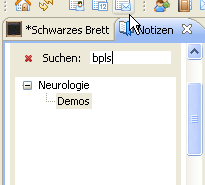
\includegraphics{find}\\
  \caption{Eintrag suchen}\label{fig:find}
\end{figure}

Die Liste wird dann auf diejenigen Einträge limitiert, die den gesuchten Begriff entweder im Titel oder in den Stichwörtern haben. Um wieder alle anzuzeigen, klicken Sie auf das rote 'x'.


\end{document} 